\documentclass[tikz,border=10pt]{standalone}
\begin{document}
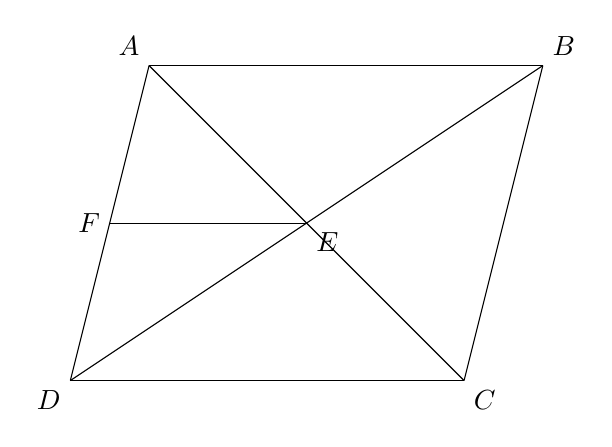
\begin{tikzpicture}
    \coordinate (A) at (1, 4);
    \coordinate (B) at (6, 4);
    \coordinate (C) at (5, 0);
    \coordinate (D) at (0, 0);
    \coordinate (E) at (3, 2);
    \coordinate (F) at (0.5, 2);

    \draw (A) -- (B);
    \draw (B) -- (C);
    \draw (C) -- (D);
    \draw (D) -- (A);
    \draw (A) -- (C);
    \draw (B) -- (D);
    \draw (F) -- (E);

    \node[above left] at (A) {$A$};
    \node[above right] at (B) {$B$};
    \node[below right] at (C) {$C$};
    \node[below left] at (D) {$D$};
    \node[below right] at (E) {$E$};
    \node[left] at (F) {$F$};
\end{tikzpicture}
\end{document}
